% !TEX program = xelatex
\documentclass[aspectratio=169,t]{beamer}
\makeatletter
\def\@makefnmark{}
\makeatletter
\usepackage{amsthm,amsmath,amssymb,braket,fontspec,unicode-math,multimedia}
\usepackage[absolute,overlay]{textpos}
\usetheme[numbering=none]{focus}
\setbeamercolor{footnote}{fg=azure}
\setbeamerfont{footnote}{size=\tiny,series=\bfseries}
\setbeamerfont{alerted text}{series=\bfseries}

\setmathfont{Latin Modern Math}[range={frak,\bigcap,\bigcup}]

\setmathfont{Latin Modern Math}[range=\checkmark]

\usepackage[backend=bibtex,url=false,doi=false,maxcitenames=1, style=authoryear]{biblatex}
\bibliography{bib}
\AtBeginBibliography{\scriptsize}

\newcommand{\focus}[1]{\textcolor{red}{\bf{#1}}}
\AtBeginSection[]{}
\definecolor{red}{HTML}{CC0000}
\definecolor{lred}{HTML}{e24a33}
\definecolor{bgreen}{HTML}{006A4E}
\definecolor{azure}{HTML}{007fff}
\newcommand{\alertb}[1]{\color{azure}\alert{#1}}
\setbeamertemplate{bibliography item}[triangle]

\graphicspath{{./figures/}}

%\AtBeginSection[]{
%  \vfill
%  \centering
%  \begin{beamercolorbox}[sep=20pt,rounded=true,center]{frametitle}
%    \usebeamerfont{title}\insertsectionhead\par%
%  \end{beamercolorbox}
%  \vfill
%}
\title{\LARGE Emergence in correlated fermions: From impurity models to the bulk}

\author{\textbf{Abhirup Mukherjee}\\\alert{RPC Presentation 2022-2023}}
\institute{\textbf{Emergent Phenomena in Quantum Matter} Group\\
Department of Physical Sciences, IISER Kolkata}

\date{July 11, 2023}
\begin{document}

\centering

\begin{frame}
\maketitle
\begin{textblock*}{0.13\textwidth}(13.5cm, 4.3cm)
	\centering

	\includegraphics[width=\textwidth]{epqm_logo_mod.jpeg}\\
	\vspace*{\fill}
	\includegraphics[width=\textwidth]{dps_logo.jpeg}
\end{textblock*}
\end{frame}

\begin{frame}{}
\hspace*{\fill}
\begin{minipage}{0.1\textwidth}
	\includegraphics[width=\textwidth]{epqm_logo_mod.jpeg}
\end{minipage}
\begin{minipage}{0.22\textwidth}
	\centering
	\includegraphics[width=0.6\textwidth]{slal.jpg}\\
	\footnotesize{{\bf Siddhartha Lal}\\
	}
\end{minipage}
\begin{minipage}{0.22\textwidth}
	\centering
	\includegraphics[width=0.6\textwidth]{amukherjee.jpg}\\
	\footnotesize{{\bf Anirban Mukherjee}\\
	}
\end{minipage}
\begin{minipage}{0.22\textwidth}
	\centering
	\includegraphics[width=0.6\textwidth]{spatra.jpeg}\\
	\footnotesize{{\bf Siddhartha Patra}\\
	}
\end{minipage}
\begin{minipage}{0.1\textwidth}
	\includegraphics[width=\textwidth]{dps_logo.jpeg}
\end{minipage}
\hspace*{\fill}
\\
\vspace*{\fill}
\begin{minipage}{0.1\textwidth}
\includegraphics[width=\textwidth]{IISER-K.png}
\end{minipage}
\hspace*{\fill}
\begin{minipage}{0.6\textwidth}
\centering
\alert{$\sim\sim\sim\sim\sim\sim\sim\sim\sim\sim\sim\sim\sim\sim\sim$ }\\
\alert{A huge thanks to all my collaborators! }\\
\alert{Thanks to IISER K and SERB for financial support.}\\
\alert{$\sim\sim\sim\sim\sim\sim\sim\sim\sim\sim\sim\sim\sim\sim\sim$ }\\
\end{minipage}
\hspace*{\fill}
\begin{minipage}{0.15\textwidth}
\includegraphics[width=\textwidth]{SERB.png}
\end{minipage}
\vspace*{\fill}

\hspace*{\fill}
\begin{minipage}{0.1\textwidth}
	\includegraphics[width=\textwidth]{IITKGP.png}\\
\end{minipage}
\hspace*{\fill}
\begin{minipage}{0.3\textwidth}
	\centering
	\includegraphics[width=0.4\textwidth]{arghya.jpg}\\
	\footnotesize{{\bf Arghya Taraphder}\\
	IIT Kharagpur}
\end{minipage}
\hspace*{\fill}
\begin{minipage}{0.3\textwidth}
	\centering
	\includegraphics[width=0.4\textwidth]{nsv.jpeg}\\
	\footnotesize{{\bf N. S. Vidhyadhiraja}\\
	JNCASR Bangalore}
\end{minipage}
\hspace*{\fill}
\begin{minipage}{0.1\textwidth}
	\includegraphics[width=\textwidth]{JNCASR.png}\\
\end{minipage}
\hspace*{\fill}

\end{frame}

\section{List of completed and ongoing projects}
\subsection{~}

\begin{frame}{List of publications, preprints and ongoing projects}
\only<1-2>{
\begin{itemize}
	\item[$\checkmark$] \onslide<1->{Unveiling the Kondo cloud: Unitary RG study of the Kondo model.\\  2022 \alert{Phys. Rev. B} 105, 085119.\\ A Mukherjee, \alert{Abhirup Mukherjee}, N. S. Vidhyadhiraja, A. Taraphder, S Lal\\[10pt]}
	\item[$\checkmark$] \onslide<1->{Frustration shapes multi-channel Kondo physics: a star graph perspective.\\  2023 \alert{J. Phys.: Condens. Matter} 35 315601. \\ S Patra, \alert{Abhirup Mukherjee}, A Mukherjee, N. S. Vidhyadhiraja, A Taraphder, S Lal\\[10pt]
	}
\item \onslide<2->{Kondo frustration via charge fluctuations: a route to Mott localisation.\\  2023 arXiv:2302.02328. \alert{under review} at New Journal of Physics.\\ \alert{Abhirup Mukherjee}, N. S. Vidhyadhiraja, A. Taraphder, S Lal\\[10pt]}
\item \onslide<2->{Holographic entanglement renormalisation for fermionic quantum matter.\\ 2023 arXiv:2302.10590. \alert{under review} at Journal of HEP.\\ \alert{Abhirup Mukherjee}, S Patra, S Lal
	}
\end{itemize}
}
\only<3>{
\flushleft
\alert{Currently in progress}\\
\begin{itemize}
	\item Development of auxiliary model-based method for studying bulk correlated systems.\\[10pt]
	\item Studies of the plateau-to-plateau transition in integer quantum hall systems.
\end{itemize}

\vspace*{\fill}
\hrule

\vspace*{\fill}
\begin{minipage}{0.55\textwidth}
\begin{itemize}
	\item[$\checkmark$] 2022 \alert{Phys. Rev. B} 105, 085119.\\ A Mukherjee, \alert{Abhirup Mukherjee}, \ldots, S. Lal\\[10pt]
	\item[$\checkmark$] 2023 \alert{J. Phys.: Condens. Matter} 35 315601.\\ S Patra, \alert{Abhirup Mukherjee}, \ldots, S. Lal
\end{itemize}
\end{minipage}
\begin{minipage}{0.44\textwidth}
\begin{itemize}
	\item 2023 \alert{arXiv:2302.02328}.\\ \alert{Abhirup Mukherjee}, \ldots, S. Lal\\[10pt]
	\item 2023 \alert{arXiv:2302.10590}.\\ \alert{Abhirup Mukherjee}, \ldots, S. Lal
\end{itemize}
\end{minipage}
}

\end{frame}

\section{Quantum phase transition in an extended-SIAM}
\subsection{Abhirup Mukherjee, N. S. Vidhyadhiraja, A. Taraphder, Siddhartha Lal\\ arXiv:2302.02328. (2023)}

\begin{frame}{Some broad questions}
\only<1>{
\footcite{georges1996,anderson_1961}
\begin{minipage}{0.4\textwidth}
Dynamical mean-field theory shows \alert{metal-insulator transition} for the Hubbard model in \(\infty\) dimensions.
\end{minipage}
\hspace*{\fill}
\begin{minipage}{0.55\textwidth}
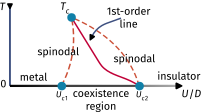
\includegraphics[width=0.8\textwidth]{coexistence-dmft.pdf}
\end{minipage}

\vspace*{\fill}
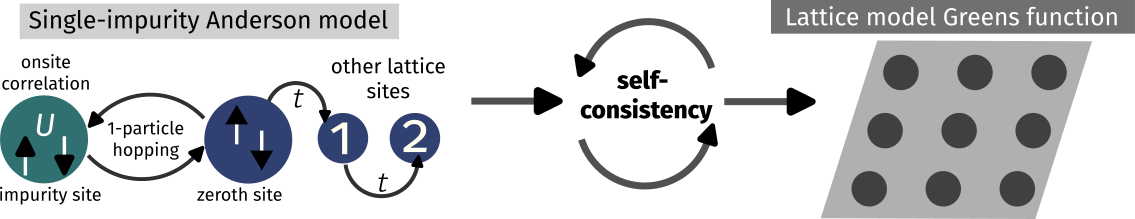
\includegraphics[width=\textwidth]{selfconsistency.pdf}
}

\only<2>{
\footcite{wilson1975,andrei_1980,Wiegmann_1981}
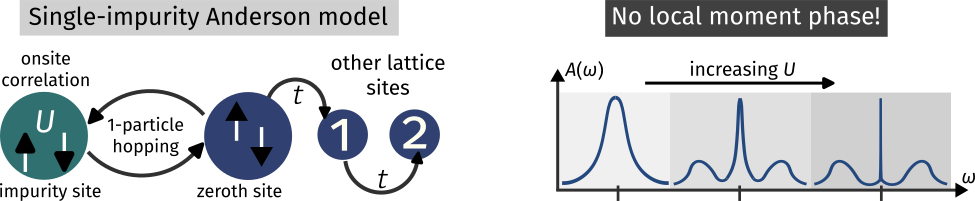
\includegraphics[width=\textwidth]{siam_schematic.pdf}

\vspace*{\fill}
Standard Anderson model shows \alert{no transition}, can't explain DMFT phase diagram.

\vspace*{\fill}
\begin{itemize}
	\item Which impurity model is realised through \alert{self-consistency}?\\[10pt]
	\item What physics leads to \(U_{c1}\) and \(U_{c2}\)?\\[10pt]
	\item What is the state precisely at the \(T=0\) \alert{transition}?
\end{itemize}
}

\end{frame}

\begin{frame}{Results}
\begin{minipage}{0.47\textwidth}
\only<1>{
	Phase \alert{transition} occurs upon adding
\begin{itemize}
	\item spin-flip correlation between impurity and bath
	\item \alert{local correlation} on bath zeroth site
\end{itemize}
}
\only<2-3>{
\begin{itemize}
	\item Local spectral function shows gap.\\[10pt]
	\onslide<3>{\item Spin correlations vanish, \alert{pairing correlations} grow at the transition}
\end{itemize}
}
\only<4-5>{
\begin{itemize}
	\item Quantum critical point shows \alert{long-ranged correlations}.\\[10pt]
	\onslide<5>{\item Excitations at the QCP are non-Fermi liquid in nature.}
\end{itemize}
}
\end{minipage}
\begin{minipage}{0.5\textwidth}
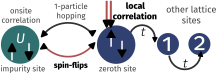
\includegraphics[width=\textwidth]{esiam-schematic.pdf}
\end{minipage}

\onslide<2-5>{
\vspace*{\fill}
\only<2-3>{
\includegraphics[width=0.45\textwidth]{spectral-function.pdf}
\onslide<3>{
\hspace*{\fill}
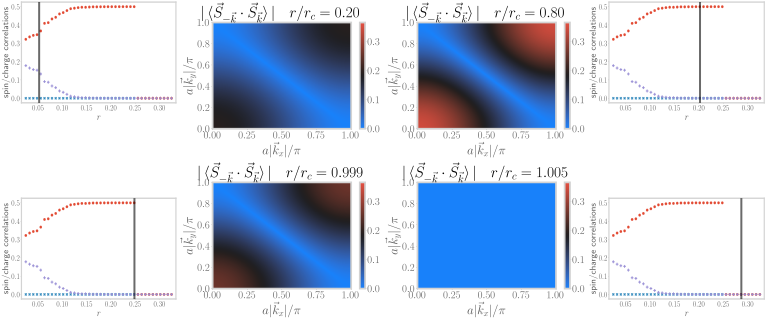
\includegraphics[width=0.45\textwidth]{spin-charge-corr-full.pdf}
}
}
\only<4-5>{
\includegraphics[width=0.45\textwidth]{rc2-spinspin-corr-di.pdf}
\includegraphics[width=0.45\textwidth]{rc2-mut-info-bath.pdf}
}
}

\end{frame}

\section{Holography of entanglement in 2D free fermions}
\subsection{Abhirup Mukherjee, Siddhartha Patra, Siddhartha Lal\\ arXiv:2302.10590. (2023)}

\begin{frame}{Some broad questions}
\footcite{Arias_2015,zaanen_2015}
\begin{minipage}{0.65\textwidth}
We consider 2D electrons placed on a torus in a flux \(\Phi\).
\begin{itemize}
	\item Is the entanglement content of this system \alert{holographic}?\\[10pt]
	\item Is there any \alert{topological} notion within the entanglement measures?
\end{itemize}
\end{minipage}
\hspace*{\fill}
\begin{minipage}{0.3\textwidth}
	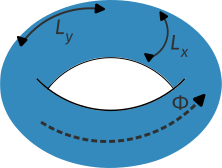
\includegraphics[width=\textwidth]{torus.pdf}
\end{minipage}

\vspace*{\fill}
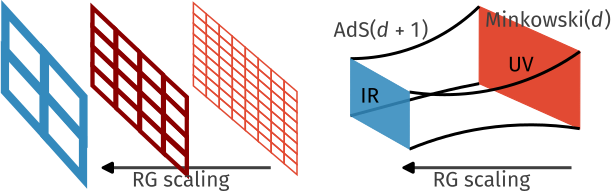
\includegraphics[width=0.8\textwidth]{holography.pdf}
\end{frame}

\begin{frame}{Results}

\begin{itemize}
	\item Choose subsystem in real space (red region)
	\item Apply \alert{coarse-graining transformations} in \(k-\)space
\end{itemize}

\vspace*{\fill}
Evolution of subspace entanglement shows interesting properties.

\vspace*{\fill}
\includegraphics[width=0.3\textwidth]{subsystem-torus.pdf}
\hspace*{\fill}
\includegraphics[width=0.5\textwidth]{coarse-graining.pdf}
\end{frame}

\begin{frame}{Results}
\footcite{van2010building,Patra2023}
\begin{minipage}{0.53\textwidth}
	Use mutual information \(I_2\) to define \alert{distance}.
\begin{itemize}
	\item Larger \(I_2\) \(\Longrightarrow\) smaller distance\\[10pt]
	\item Allows notion of \alert{curvature} as well.\\[10pt]
\end{itemize}
Coarse-graining transformations lead to \alert{emergent} spatial dimension
\end{minipage}
\hspace*{\fill}
\begin{minipage}{0.43\textwidth}
	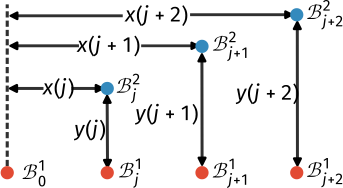
\includegraphics[width=\textwidth]{curvature-scheme.pdf}
\end{minipage}

\onslide<2>{
\vspace*{\fill}
\begin{minipage}{0.4\textwidth}
	\includegraphics[height=0.25\textheight]{Matroshka.png}
	\includegraphics[height=0.25\textheight]{nested.png}
\end{minipage}
\hspace*{\fill}
\begin{minipage}{0.55\textwidth}
Other consequences:
\begin{itemize}
	\item \alert{hierarchy} of entanglement exists along the RG
	\item hierarchy also present in \alert{multipartite entanglement}
\end{itemize}
\end{minipage}
}
\end{frame}

\begin{frame}{Results}
\footcite{oshikawa2000topological,seki2017topological,alexandradinata_2011}
\begin{minipage}{0.63\textwidth}
\begin{itemize}
	\item By tuning flux, we relate Luttinger's volume to functions of entanglement
	\item Entanglement spectral flow is also related to Chern numbers in presence of magnetic field
\end{itemize}
\end{minipage}
\hspace*{\fill}
\begin{minipage}{0.35\textwidth}
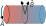
\includegraphics[width=\textwidth]{cylinder.pdf}
\end{minipage}

\vspace*{\fill}
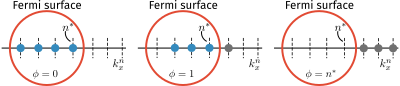
\includegraphics[width=\textwidth]{spectral-flow.pdf}
\end{frame}

\section{Tiling a lattice with the extended SIAM}
\subsection{Ongoing project}

\begin{frame}{Broad questions}

\vspace*{\fill}
\begin{minipage}{0.5\textwidth}
\begin{itemize}[<+->]
	\item Studying the \alert{Mott MIT} on the 2D Hubbard-Heisenberg model\\[10pt]
	\item Obtaining a \alert{momentum-space} picture of the transition.\\[10pt]
	\item Devising a method to tackle lattice models \alert{using impurity models}
\end{itemize}
\end{minipage}
\hspace*{\fill}
\begin{minipage}{0.4\textwidth}
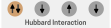
\includegraphics[width=\textwidth]{hubbard.pdf}
\end{minipage}

\vspace*{\fill}
\end{frame}

\begin{frame}{Results}
\flushleft
We use impurity model eigenstates (Hamiltonians) and \alert{Bloch's theorem} to reconstruct full eigenstates (Hamiltonian):
\[\ket{\Psi_{\vec k}} \sim \sum_{\vec R_i} e^{i \vec{k}\cdot\vec{R}_i} \ket{\psi_\text{aux}(\vec R_i)},\quad\mathcal{H} \sim \sum_{\vec R_i} \mathcal{H}_\text{aux}(\vec R_i)\]
\vspace*{\fill}
\only<1>{
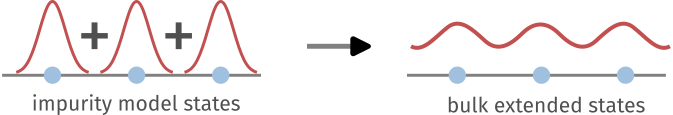
\includegraphics[width=\textwidth]{bloch.pdf}
}
\only<2>{
\flushleft
Allow us to \alert{relate corresponding objects} between the impurity model and the lattice model\\
\begin{itemize}
	\item Greens functions and self-energies\\[10pt]
	\item Two-particle correlation functions\\[10pt]
	\item entanglement measures 
\end{itemize}
}
\end{frame}

\begin{frame}{Results: Momentum space spectral function}
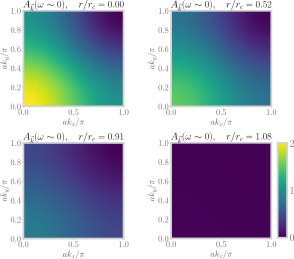
\includegraphics[width=\textwidth]{kspace-spectralfunction-all.pdf}
\end{frame}

\begin{frame}{Results: Momentum space spin correlations}
\hspace*{-22pt}
\includegraphics[width=1.1\textwidth]{kspace_corr.pdf}
\end{frame}

\section{Search for punctured-Chern topology at IQHE transitions}
\subsection{Ongoing project}

\begin{frame}{Broad questions}

\vspace*{\fill}
\begin{minipage}{0.5\textwidth}
\begin{itemize}[<+->]
	\item Obtaining the \alert{IQHE phase diagram} from a model of 2D lattice electrons\\[10pt]
	\item Understanding the \alert{topology} of the ground state precisely at a transition\\[10pt]
	\item Extending this to systems with \alert{disorder}.
\end{itemize}
\end{minipage}
\hspace*{\fill}
\begin{minipage}{0.4\textwidth}
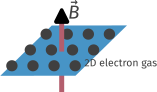
\includegraphics[width=\textwidth]{IQHE.pdf}
\end{minipage}

\vspace*{\fill}
\end{frame}

\begin{frame}{Preliminary results}
Emergence of \alert{Landau levels} in a magnetic field is similar to the formation of \alert{bands} in a periodic potential.

\vspace*{\fill}
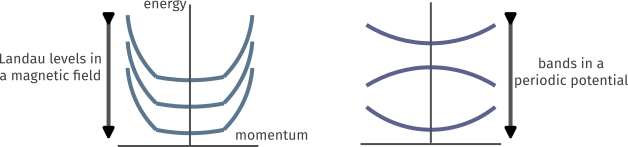
\includegraphics[width=\textwidth]{bands.pdf}

\vspace*{\fill}
We first studied the simpler problem of \alert{particle in a periodic potential}.
\end{frame}

\begin{frame}{Preliminary results}
We first studied the simpler problem of \alert{particle in a periodic potential}.

\vspace*{\fill}
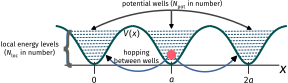
\includegraphics[width=0.8\textwidth]{potential.pdf}

\vspace*{\fill}
	
\begin{itemize}
	\item Can understand the formation of bands under RG
	\item Obtained insights regarding the \alert{effective center of mass} degrees of freedom
	\item Needs to be extended by incorporating a \alert{magnetic field}
\end{itemize}
\end{frame}

\section{Summary}
\subsection{~}

\begin{frame}{Summary}
\alert{Currently in progress}\\
\begin{itemize}
	\item Development of auxiliary model-based method for studying bulk correlated systems.\\[10pt]
	\item Studies of the plateau-to-plateau transition in integer quantum hall systems.
\end{itemize}

\vspace*{\fill}
\hrule

\vspace*{\fill}
\begin{minipage}{0.55\textwidth}
\begin{itemize}
	\item[$\checkmark$] 2022 \alert{Phys. Rev. B} 105, 085119.\\ A Mukherjee, \alert{Abhirup Mukherjee}, \ldots, S. Lal\\[10pt]
	\item[$\checkmark$] 2023 \alert{J. Phys.: Condens. Matter} 35 315601.\\ S Patra, \alert{Abhirup Mukherjee}, \ldots, S. Lal
\end{itemize}
\end{minipage}
\begin{minipage}{0.44\textwidth}
\begin{itemize}
	\item 2023 \alert{arXiv:2302.02328}.\\ \alert{Abhirup Mukherjee}, \ldots, S. Lal\\[10pt]
	\item 2023 \alert{arXiv:2302.10590}.\\ \alert{Abhirup Mukherjee}, \ldots, S. Lal
\end{itemize}
\end{minipage}

\end{frame}

\section{Future plans}
\subsection{~}

\begin{frame}{Future plans}
\only<1>{
\footcite{keimer2015quantum,qin_2022}
\begin{minipage}{0.6\textwidth}
\alert{Lattice models of impurities}
\begin{itemize}
	\item either directly or through the auxiliary model approach\\[10pt]
	\item phase diagrams: strange metals and QCPs\\[10pt]
	\item unconventional superconductivity
\end{itemize}
\end{minipage}
\hspace*{\fill}
\begin{minipage}{0.35\textwidth}
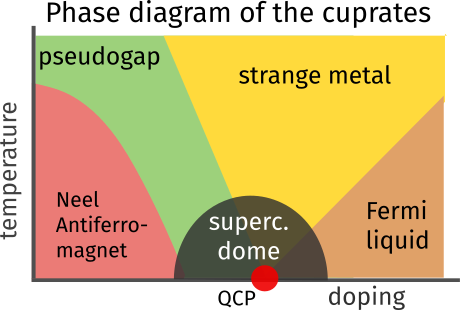
\includegraphics[width=\textwidth]{cuprates.pdf}
\end{minipage}

\vspace*{\fill}
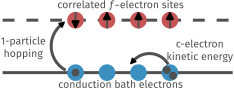
\includegraphics[width=0.5\textwidth]{periodicAnderson.pdf}
}
\only<2>{
\alert{Fractional Chern insulators}\\[5pt]
\begin{itemize}
	\item microscopic understanding of the FQHE ground states\\[10pt]
	\item emergence of composite degrees of freedom and topological theories
\end{itemize}

\vspace*{\fill}
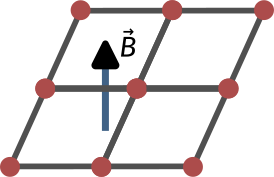
\includegraphics[width=0.3\textwidth]{ChernInsulator.pdf}
}
\only<3>{
\alert{Classification of RG flows in fermionic models}\\[5pt]
\begin{itemize}
	\item growth of multipartite entanglement towards stable fixed points\\[10pt]
	\item extending this to impurity models\\[10pt]
	\item connections with the URG noise operator
\end{itemize}
}
\end{frame}

\begin{frame}[c]{}
	\LARGE{THANK YOU.}
\end{frame}

\end{document}
